% -*- root: ../GeometriaDiferencial.tex -*-
\section{Diferentiable Manifolds}

\begin{problem}[1]
Show with details that the real projective space is a differentiable manifold

\solution
\textcolor{blue}{Este ejercicio está prácticamente resuelto en teoría pero lo repetimos aquí con más detalle}

Recordamos que, por definición, un conjunto $X$ es una variedad diferenciable si cumple:
\begin{enumerate}
\item $X$ es un espacio topológico con topología conexa y Hausdorff\footnote{Ver magníficos apuntes de Topología I.}.
\item $U_i ⊂ X$ es una familia numerable de abiertos con aplicaciones $\appl{Φ_i}{U_i}{ℝ^n}$, homomorfismos sobre sus imágenes. El par $(U_i, Φ_i)$ es una carta coordenada.
\item Para todo par de de cartas coordenadas $U_i, U_j$ de la estructura diferencial\footnote{Una variedad queda unívocamente definida por un atlas maximal. Un atlas maximal es un atlas que contiene a todos los atlas que son compatibles con él. Dos atlas son compatibles si son equivalentes} y sus correspondientes homomorfismos $Φ_i, Φ_j$, la función $ \inv{Φ_i} ○ Φ_j $ es difeomorfismo en el entorno en el que está definida (en $U_i ∩ U_j$).
\end{enumerate}

Por otro lado tenemos el plano proyectivo definido como:
\[ \projp^2 ≝ \quot{ℝ^3 \setminus \set{0}}{\sim} \]
donde $\sim$ es una relación de equivalencia definida de la siguiente forma: dados $e, e' ∈ ℝ^3$, están relacionados $e \sim e'$ si y sólo si $∃λ ≠ 0$ tal que $λe = e'$.

Primero hay que dotar de una topología a este espacio. Para ello vamos a definir unos conjuntos:

\[U_i = \{(x_1,x_2,x_3) : x_i ≠ 0\}\]

Esta construcción permite decir que $\projp^2(ℝ) = \displaystyle\bigcup_{i=1}^3 U_i$. En cada conjunto se puede construir el homomorfismo $\appl{Φ_i}{U_i}{ℝ^2}$ llevando $[x_0, x_1, x_2]$ a $\left[\frac{x_0}{x_i},\frac{x_1}{x_i},\frac{x_2}{x_i}\right]$. Dado que una de las coordenadas va a ser $1$ siempre, podemos quitarla y entonces será equivalente a $ℝ^2$.

Definimos la topología del plano proyectivo como:

\[ A⊂U_i, A∈\topl \dimplies Φ_i(A) ∈\topl_{ℝ^n}\]

es decir, un subconjunto de $U_i$ es abierto si y sólo si su imagen por $Φ_i$ es un abierto en $ℝ^n$ con la topología habitual. No es de este curso comprobar que esto realmente define una topología ni que esta topología sea la topología con más abiertos tal que la aplicación $\appl{π}{\real^3 \setminus \set{0}}{\projp^2}$ es continua\footnote{$π$ es la combinación apropiada de $Φ_i$ para que sea continua. Es como la proyección en el plano proyectivo utilizado todas las $Φ_i$}.

Esta topología es conexa y Hausdorff, y también compacta.

Al tener una topología conexa y Hausdorff, el plano proyectivo es una variedad topológica.

Tendríamos que comprobar la tercera propiedad de variedad diferenciable. Para ello vemos que el plano proyectivo tratado como variedad tiene tres cartas, dadas por $(U_i,Φ_i)$.

Si tomamos dos cartas $(U_i, Φ_i), \ (U_j, Φ_j)$ vemos que la intersección de los $U$ es:
\[W = U_i \cap U_j= \{(x_1,x_2,x_3): \ x_i \neq 0 \ x_j \neq 0\}\]

Veamos como se comporta la aplicación $ \inv{Φ_i} ○ Φ_j $  sobre $W$:
\[\inv{Φ_i} ○ Φ_j (W)= \inv{Φ_i} \left(\left\{ \left(\frac{x_1}{x_j}, \frac{x_2}{x_j},\frac{x_3}{x_j}\right)\right\}\right) = \left\{ \left(\frac{x_i \cdot x_1}{x_j}, \frac{x_i \cdot x_2}{x_j},\frac{x_i \cdot x_3}{x_j}\right)\right\} \text{ con } i,j \in \{1,2,3\}\]

Puesto que partimos de la premisa de que $x_i, x_j \neq 0$ tenemos que la función es claramente diferenciable\footnote{cada coordenada es un polinomio de varias variables con un posible denominador no nulo} y puede comprobarse fácilmente que es biyectiva.

La inversa de esta función sería $ Φ_i ○ \inv{Φ_j}$ que se comportaría de la siguiente forma:
\[Φ_i ○ \inv{Φ_j}\left( \{(y_1, y_2, y_3)\}\right) =Φ_i  \left( \{y_1x_j, y_2x_j, y_3x_j\}\right) = \left\{ \left(\frac{y_1x_j}{x_i}, \frac{y_2x_j}{x_i}, \frac{y_3x_j}{x_i} \right)\right\}\]

Esta función sólo estará definida en aquellos puntos en que $x_i\neq$ por lo que resulta ser también diferenciable y vuelve a ser sencilla la comprobación de que la función es biyectiva por lo que queda claro que es un difeomorfismo y por tanto \textbf{el plano proyectivo es una variedad diferencial}

\end{problem}

\begin{problem}[3]
Let $\appl{γ}{M}{N}$ be a differentiable map. Show that the definition of the differential $\appl{dγ_p}{\tgs_p M}{\tgs_{γ(p)} N}$ ofγ at $p$ does not depend on the choice of the curve and that $dγ_p$ is a linear map.

\solution
\textcolor{blue}{Hecho por Pedro. No fiarse al 100\%}

Por definición tenemos
\[dγ_p(v) \in \tgs_{α(p)} N = (γ\circ α)'(0)\]
siendo
\[\appl{α}{(-ε, ε)}{M} \text{ con } α(0)=p, α'(0)=v\]

Sabemos que
\[(γ\circ α)'(0) = α'(0)(γ'(α(0)) = v \cdot γ'(p)\]

sin importar la curva $α$ tomada siempre y cuando cumpla las condiciones pedidas.

Ahora es sencillo ver que es lineal pues tenemos que es una aplicación que, dado un vector $v$ nos lleva a ese mismo vector multiplicado por un valor constante por lo que es lineal de manera trivial.
\end{problem}

\begin{problem}[4]
Let $\appl{γ}{M}{N}$ be an inmersion and let $p$ be a point in $M$. Show that there exists a neighborhood $V \subset M$ of $p$ such that the restriction $γ|_V$ is an embedding (This means that every inmersion is locally an embedding).

\solution
\textcolor{blue}{Hecho por Pedro. No fiarse al 100\%}

Para empezar recordemos lo que era una \textbf{inmersión}: Sean $M$ y $N$ variedades diferenciables. Se dice que una función diferenciable $\appl{F}{M}{N}$ es una \textbf{inmersión} en $p$ si la diferencial $\appl{F_{*p}}{\tgs_pM}{\tgs_{F(p)}N}$ entre los espacios tangentes es inyectiva. Si $F$ es una inmersión para todo punto $p\in M$ decimos que es una \textbf{inmersión}.

Recordemos también lo que era un \textbf{embedding}: Si una \textbf{inmersión} es un homeomorfismo sobre su imagen, con la topología inducida en esta por $N$, decimos que es un \textbf{embedding}

Puesto que toda función diferenciable es continua podemos tomar un entorno de $γ(p)$ y calcular su preimagen, que será un entorno de $p$. La restricción de γ a este entorno será inyectiva, por ser inyectiva γ en general y será sobreyectiva por construcción por lo que será biyectiva. Así podemos garantizar que tendrá inversa diferenciable y por tanto se trata de un homeomorfismo sobre su imagen lo que implica que γ es un \textbf{embedding}
\end{problem}
\newpage
\begin{problem}[6]
Consider the cylinder $C=\{(x,y,z) \in \real^3 \tq x^2+y^2=1\}$ and indentify the point $(x,y,z)$ with $(-x,-y,-z)$. Show that the quotient space of $C$ by this equivalence relation can be given a differentiable structure. (infinite Möbius band)
\solution

\textcolor{blue}{Hecho por Pedro. No fiarse al 100\%}

Primero mostramos un ejemplo encontrado por internet que resuelve un problema muy similar a este.

\begin{center}
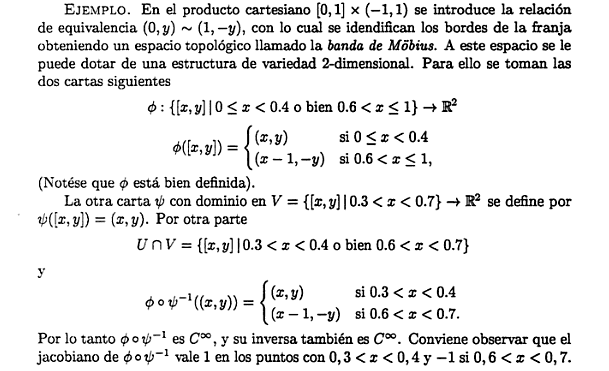
\includegraphics[keepaspectratio=true,width=\linewidth]{img/ejemplo_6.png}
\end{center}

Para dotar a un conjunto de estructura diferencial basta con encontrar un atlas para el cual se cumpla la definición de estructura diferencial sobre el conjunto dado.

Tomamos 8 cartas de la siguiente forma:
\begin{enumerate}
\item
\[\appl{\phi_1}{\{(x,y,z) \tq x\in [0,1), y \in [0,1), z \geq 0\}}{\real^3}\]
siendo $\phi_1=Id$
\item
\[\appl{\phi_2}{\{(x,y,z) \tq x\in (-1,0], y \in [0,1), z \geq 0\}}{\real^3}\]
siendo $\phi_2((x,y,z)=(-x,y,z)$
\item
\[\appl{\phi_3}{\{(x,y,z) \tq x\in [0,1), y \in (-1,0], z \geq 0\}}{\real^3}\]
siendo $\phi_3((x,y,z)=(x,-y,z)$
\item
\[\appl{\phi_4}{\{(x,y,z) \tq x\in [0,1), y \in [0,1), z < 0\}}{\real^3}\]
siendo $\phi_4((x,y,z)=(x,y,-z)$
\item
\[\appl{\phi_5}{\{(x,y,z) \tq x\in (-1,0], y \in (-1,0], z \geq 0\}}{\real^3}\]
siendo $\phi_5((x,y,z)=(-x,-y,z)$
\item
\[\appl{\phi_6}{\{(x,y,z) \tq x\in (-1,0], y \in [0,1), z < 0\}}{\real^3}\]
siendo $\phi_6((x,y,z)=(-x,y,-z)$
\item
\[\appl{\phi_7}{\{(x,y,z) \tq x\in [0,1), y \in (-1,0], z < 0\}}{\real^3}\]
siendo $\phi_7((x,y,z)=(x,-y,-z)$
\item
\[\appl{\phi_8}{\{(x,y,z) \tq x\in (-1,0], y \in (-1,0], z < 0\}}{\real^3}\]
siendo $\phi_8((x,y,z)=(-x,-y,-z)$

\end{enumerate}

La combinación de una de estas funciones con la inversa de otra no implicará más que cambios de signo sobre las variables de tal forma que
\[\phi_i\circ \inv{\phi_j}(x,y,z)=(\pm x, \pm y, \pm z\]
y queda claro que estas aplicaciones son $C^{\infty}$ y sus inversas, que son de la misma forma, también. Conviene observar que el jacobiano vale siempre $\pm 1$
\end{problem}

\section{fasc-4-ejemplos}

\subsection{Variedades}
\begin{problem}[1]
Demostrar con detalle las afirmaciones contenidas en los ejemplos, y, en caso particular, todas las que se refieren a la construcción de cartas coordenadas y atlas. Hacer también los ejercicios intercalados en el texto.

\solution

\end{problem}

\begin{problem}[2]
Estudiar, siguiendo el modelo de $S^2$ la estructura de variedad diferenciable, con dos cartas, en $S^n$

\solution

\end{problem}

\begin{problem}[3]
Parametrizamos los puntos del hemisferio norte de la esfera $x_2 > 0$,
excluyendo el ecuador $x_2 = 0$, en la forma $(θ, τ, + \sqrt{1 − θ^2 − τ^2})$ con
$θ^2 + τ^2 < 1$. Esto convierte al hemisferio norte en una carta coorde-
nada, y podemos cubrir la esfera con seis cartas de este tipo tomando
como ecuador cada una de las intersecciones de la esfera con los planos
coordenados. COMPROBAR que, efectivamente, se trata de un atlas.

DEMOSTRAR que los dos atlas son equivalentes, viendo que los cambios
de carta de una carta de uno de ellos a una carta del otro inducen difeo-
morfismos.

\solution
\end{problem}

\begin{problem}[4]
Demostrar que no existe ninguna variedad diferenciable compacta que se pueda recubrir con una única carta coordenada
\solution
\end{problem}

\begin{problem}[5]
Demostrar que toda variedad 1-dimensional compacta y conexa es difeomorfa a la circunferencia $S^2$
\solution

\end{problem}

\begin{problem}[6]
Demostrar, como consecuencia del teorema de invarianza del dominio, que si $n \neq m$, no pueden ser homeomorfos $\real^n$ y $\real^m$. Tampoco es posible que sean homeomorfos un abierto de $\real^n$ con uno de $\real^m$
\solution

\end{problem}
\subsection{Campos}